\section{pygrametl Reinterpreter}
In order to increase usability, we would like to allow users to give the pygrametl program they wish to test, along with some test data, to our framework. Our framework should then be able to executed the pygrametl program with the test data instead of of its normally used sources. And then return some form of representation of the resulting populated tables, that can be used later for our predicates. This approach requires us to solve some subproblems,

\begin{itemize}
\item How should the user specify their inputs to the reinterpreter?
\item How do we make changes to the pygrametl program and how can we ensure that the pygrametl program is executed correctly after these changes? 
\item How do we represent the resulting data warehouse and how do we extract it?
\end{itemize}

\begin{figure}
  \centering
  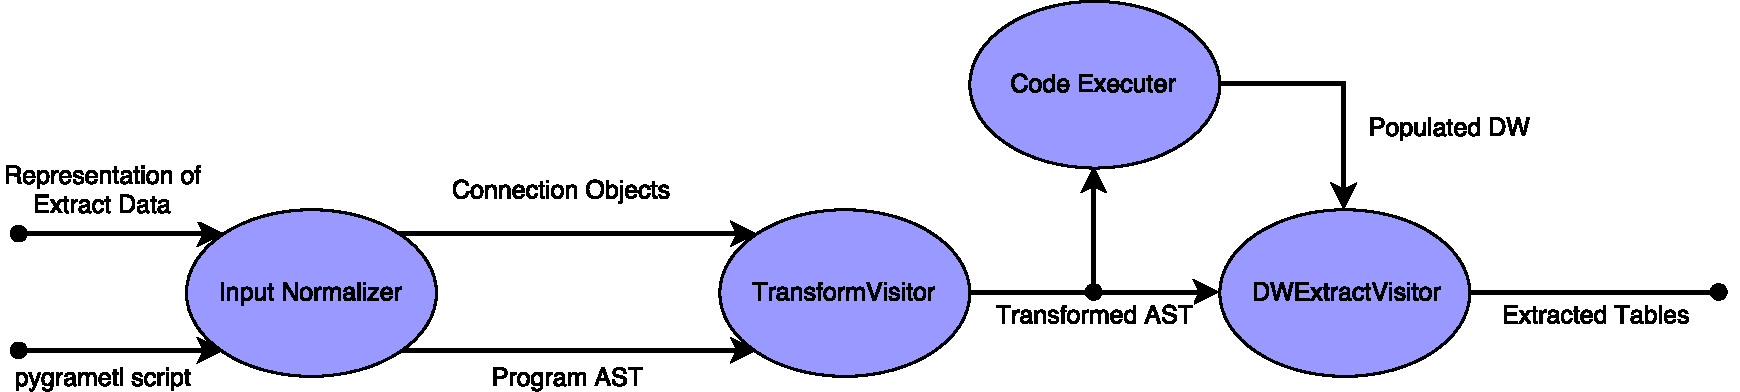
\includegraphics[width=0.5\textwidth]{figures/reinterpreter_model.pdf}
  \caption{Data model of our Reinterpreter}
\end{figure}

The rest of this section would focus on explaining how we attempt to solve these subproblems.

\subsection{Inputs for the Reinterpreter}
There are a number of inputs required for the reinterpreter to work. For one, it requires the pygrametl program that it is supposed to reinterpret. Thermore it also requires knowledge about how it is supposed to reinterpret the program. The first can be simply given as a string containing the source code of the pygrametl program or a path to a file containing the source. Giving the reinterpreter knowledge about how to reinterpret the program can be more tricky however. The knowledge we wish to give is the data used in the extract part of the etl process, and we wish to allow the user to be able to give this in an easy way. 

We see two reasonable ways of giving this, either the user can give a connection to a database, which we will then use to replace the connections used in pygrametls datasource objects. Or the user could give some form of datatype that could be coded directly in python, such as a dict, that mimics a database. The reinterpreter could then take this and create a mock database using SQLite and replace the connection in pygrametls datasources objects with one to this mock database.

Both approaches has their benefits, if the user already has made scripts that can easily populate sample databases, then simply making connections to these databases would easy. While hardcoding a datatype increases the readability of the test code, since the user doesn’t have to open a database to see the data that used in the pygrametl program.


\subsection{How to make changes to the program}
After we have given the program and what parts of it we wish to change, we have to do the actual modifications. This step is the hardest, as we would like our reinterpreter to be able to take an arbitrary pygrametl program, and then apply these changes. The problem is that there ins’t one specific way that people could use the pygrametl package. Some may use it by simply making a single file script that can be run to populate a DW, while others might implement it into some of their own packaging, spreading the functionality of pygrametl over multiple files.
We decide to simply focus on the ones who writing pygrametl programs as simple single file scripts. As this allows us to parse the file and then later execute it with relative ease. Whereas the other approach would leave too many dependencies we wouldn’t be able to handle with the use of ASTs.

So how do we make these changes to the program then? As mentioned, we first parse the program so we get the AST. This allows us to make changes to the AST instead of directly to the code, where we would have to handle a lot of syntactic sugar.  Using this approach, we should be able to identify all of the instantations of pygrametl datasource objects in the code, and then replace their connection parameters with the ones we would like instead. By changing the connection of the datasource objects, the rest of the pygrametl program should work as usual, given that the datasource objects SQL query is valid for the new connection.

Additionally we would also have to handle the ConnectionWrapper used in the pygrametl program. As should populate the normal DW with the result of the program, but rather populate a mock one that we will later test our predicates upon. This could also be done in two ways, we could either have the user specify a connection to a database that has the same schema as their DW, that we would then populate. Or they could not do the above, and we could make a database using SQLite and by extracting information regarding its schema from the instantiations of Dimension and FactTable objects in the AST.

Once all of the necessary changes have been made, we can simply compile and execute the AST using the built-in python functions compile and exec respectively.

\subsection{The resulting DW and how to extract the data from it}
